\documentclass[11pt,a4paper]{article}
\usepackage[T1]{fontenc}
\usepackage[left=3cm, right=3cm, top=3cm, bottom=3cm]{geometry}
\usepackage{graphicx}
\usepackage{mathtools}
\usepackage{amssymb}
\usepackage{amsthm}
\usepackage{thmtools}
\usepackage{nameref}
\usepackage{hyperref}
\usepackage{times}
\begin{document}
\begin{center}
		\Large \textbf{Flat Field Generation from observations.}
\end{center}
	The system wide flat field of SUIT is necessary to remove large scale patterns seen in the SUIT images. These patterns 	arise due to optical or electronic reasons. The off pointed solar images are combined as per the method described above and we get the illumination as in Figure \ref{fig:flat_field}. 
	
	Our motivation is to select size scales that affect our observations. In this case, it is a diagonal series of lines repeating at intervals of 310 pixels across the direction perpendicular to the lines. A test is performed to confirm the methodology and the procedure used to isolate the striped nature of the uneven illumination.
	
	\section{Methodology}
	\begin{itemize}
		\item Aditya is moved on roll and pitch axes in steps of 8 arc mins. The entire field of view (FOV) is covered by the solar disk with 28 pointings of the satellite.
		\item The observations are made with 11 filter combinations of SUIT over a period of 18 days.
		\item Scattered light and bias is removed from each image before processing them to generate the flat field.
		\item The images are sorted and any partial frames are discarded.
		\item On an average, approximately 14 images are obtained per filter, per pointing of SUIT.
		\item The scatter and bias corrected images are added to increase the signal to noise ratio (SNR) of the raw data. We shall call these \textit{Summation Images.}
		\item The \textit{Summation Images} are combined using the developed algorithm to create the illumination pattern. We shall call this \textit{Blended Image}.
		\item The feature scale of interest is identified. in our case, the periodic stripe like pattern is seen to repeat itself after every 620 pixels along the direction perpendicular to the stripes.
		\item We apply a boxcar blurring to remove all structures smaller than 6.5 px in size. This is necessary to get rid of the small scale fluctuations in the image due to pixel response non uniformity or small contaminants on the CCD. We shall call this \textit{Small Scale Removed Image}.
		\item A copy of the blurred image is generated. Boxcar blurring of kernel size 620 px is applied on this copy to derive the large scale non uniformity of illumination in the image. This could be arising from non uniform ilumination of the CCD due to the telescope optics, or due to limb darkening of the sun around the edges of the image. We shall call this \textit{Large Scale Illumination Profile}.
		\item The bluring kernel size of 620 pixels is derived analytically based on the frequency of the stripes appearing on the image. The methodology used for this is described ahead in the document.
		\item The \textit{Large Scale Illumination Profile} is divided from the \textit{Small Scale Removed Image} to extract the feature of our choice, the stripe like pattern.
		
	\end{itemize}
	
	
	
	\begin{figure}
		\centering
		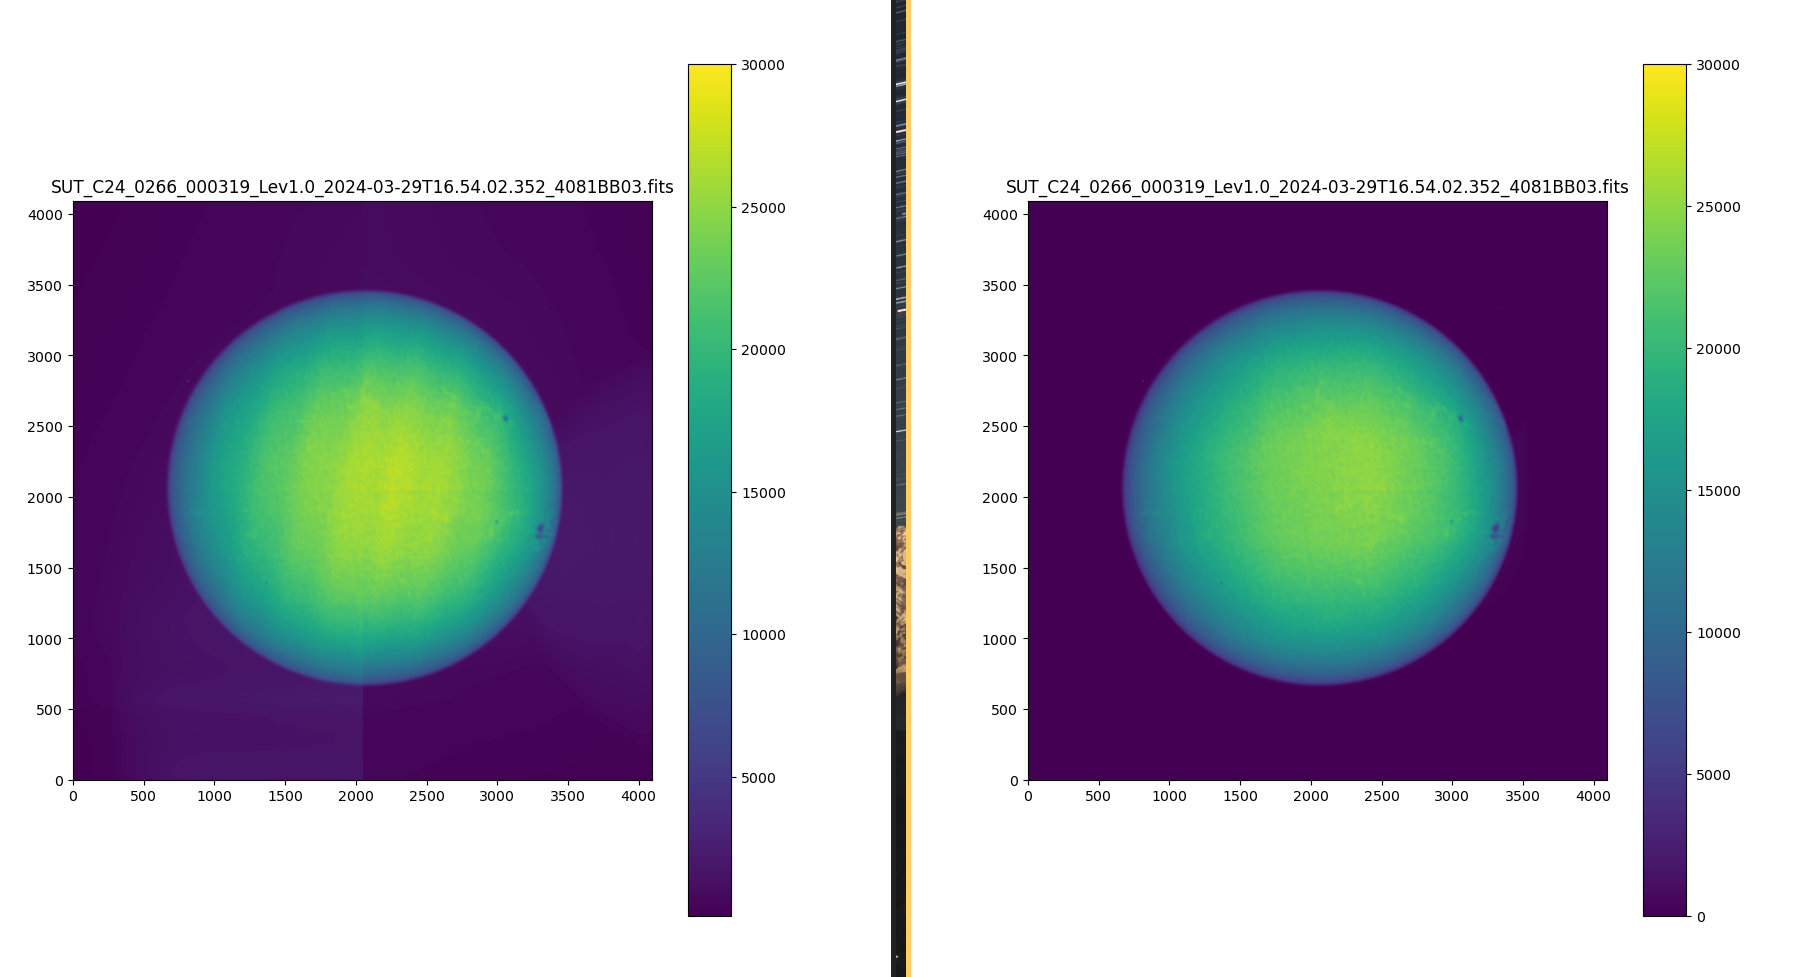
\includegraphics[width=0.7\linewidth]{pics/screenshot_2024-06-06_12-24-27}
		\caption{SUIT Image, before and after flat field correction}
		\label{fig:compare}
	\end{figure}
	
	\begin{figure}
		\centering
		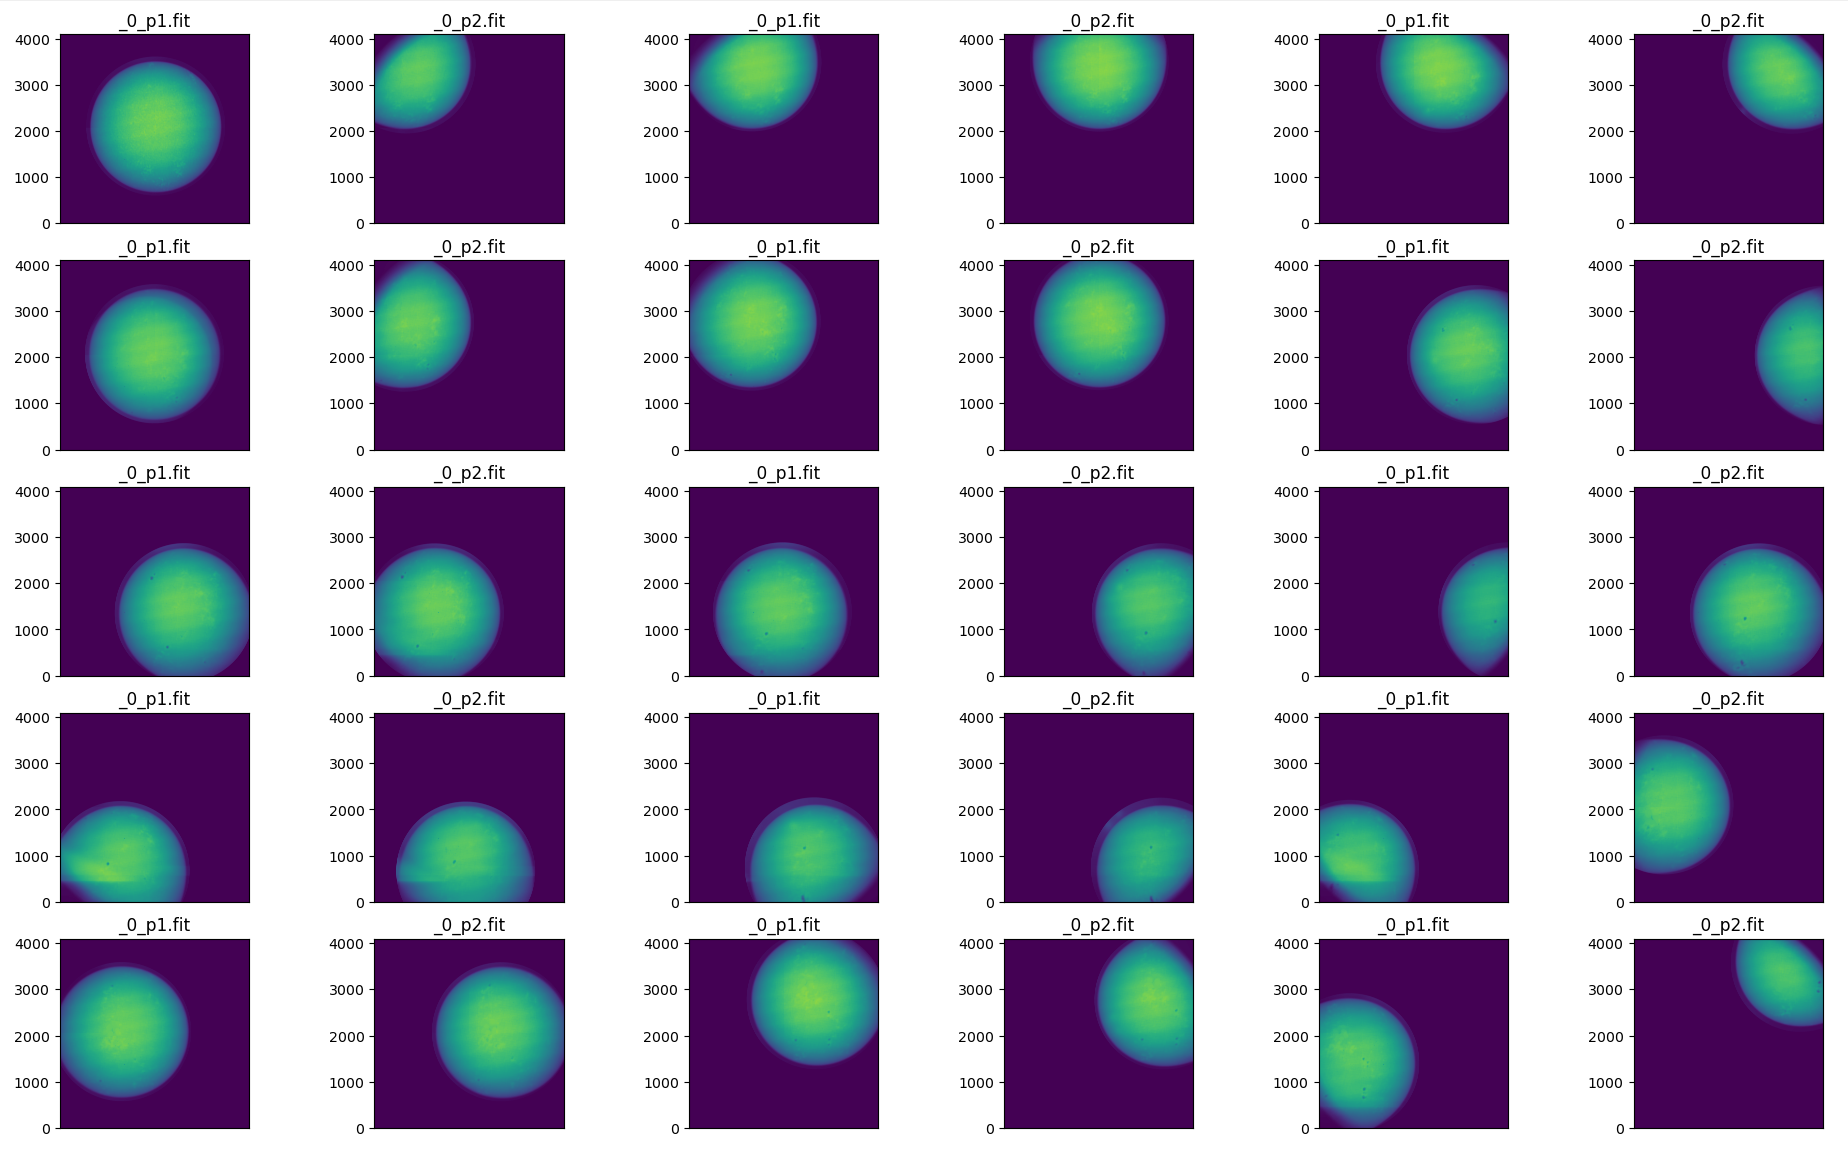
\includegraphics[width=0.7\linewidth]{pics/screenshot_2024-06-06_11-35-10.png}
		\caption{Solar off pointing- NB06 images.}
		\label{fig:off pointing}
	\end{figure}
	
	\begin{figure}
		\centering
		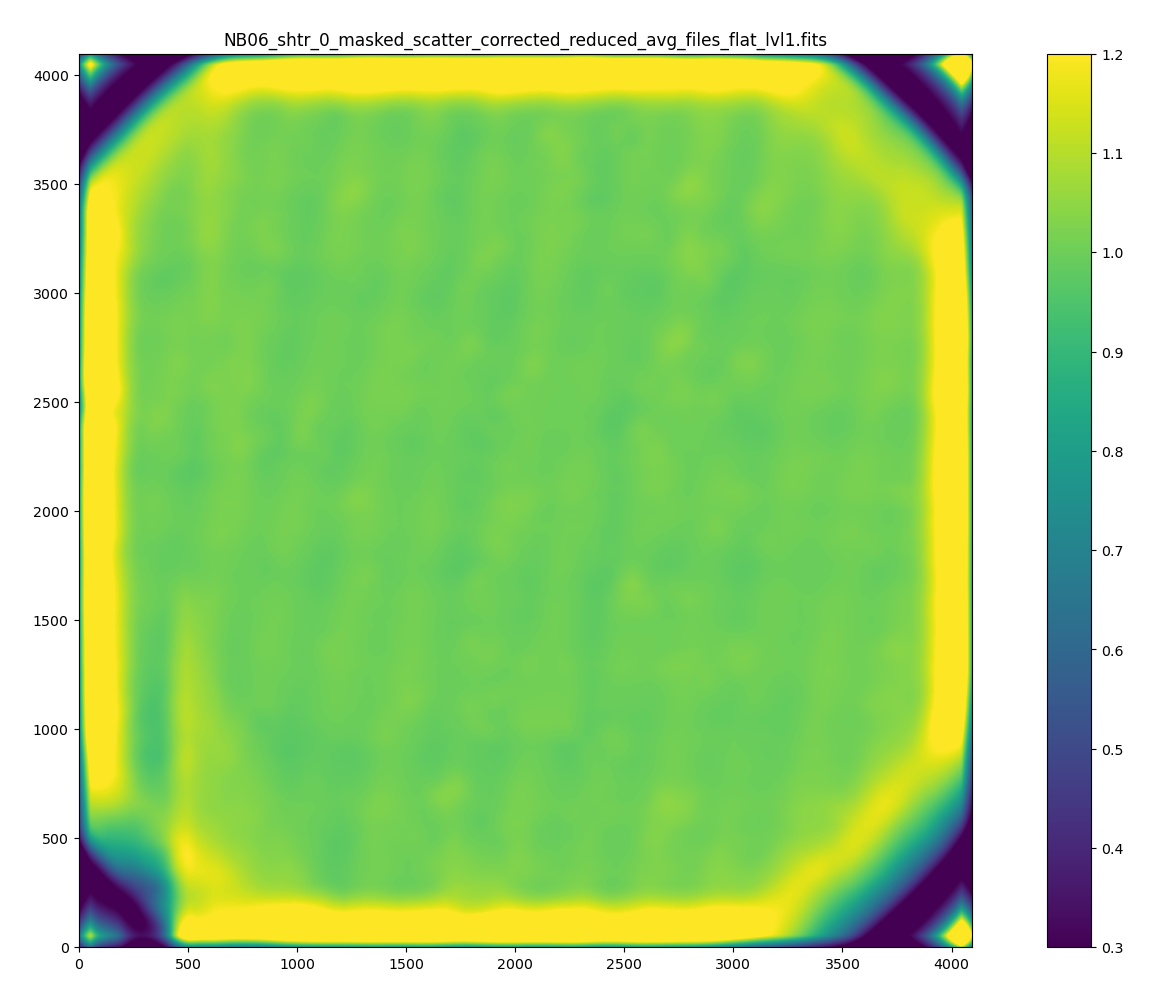
\includegraphics[width=0.7\linewidth]{pics/screenshot_2024-06-06_11-40-31.png}
		\caption{Solar off pointing- NB06 images.}
		\label{fig:flat_field}
	\end{figure}
	
	
\end{document}